\documentclass[twocolumn, a4paper]{article}

% Packages{{{
\usepackage[sc]{mathpazo}
\usepackage{graphicx}
  \graphicspath{ {./images/} }
\usepackage[T1]{fontenc}
  \linespread{1.2}
\usepackage{microtype}
\usepackage{blindtext}
\usepackage{soul}

\usepackage[english]{babel}

\usepackage[hmarginratio=1:1,top=32mm,columnsep=15pt]{geometry}
\usepackage[hang, small,labelfont=bf,up,textfont=it,up]{caption}
\usepackage{booktabs}
\usepackage{tcolorbox}

\usepackage{lettrine}

\usepackage{enumitem}
  \setlist[itemize]{noitemsep}

\usepackage{titlesec}
\titleformat{\section}[block]{\Large\scshape\centering}{}{0em}{}
\titleformat{\subsection}[block]{\large}{}{0em}{\textbf}
\titleformat{\subsubsection}[block]{}{}{0em}{\textbf}
\titleformat{\part}[block]{\Huge\scshape\centering}{}{0em}{}


\usepackage{titling}
\usepackage{hyperref}
%}}}
% Title{{{
\setlength{\droptitle}{-4\baselineskip}

\pretitle{\begin{center}\Huge\bfseries}
\posttitle{\end{center}}
\title{Internet Technology}
\author{ by
  \textsc{Swapnil}%\\[1px]
}
\date{}
%}}}

\begin{document}
% FontMatter {{{
% \begin{titlingpage}
  \maketitle
  % \thispagestyle{empty}
  % \setcounter{tocdepth}{3}
  % \tableofcontents
% \end{titlingpage} }}}

\begin{tcolorbox}
  \part{Unit 1}
\end{tcolorbox}
\section{E-mail Address}
An email address is a designation for an electronic mailbox that sends and
receives messages, known as email, on a computer network. Since the 1980s, all
email addresses follow the same format: @. An example is below.

\begin{center}
  \verb+janedoe@domainname.com+
\end{center}
On the far right, the .com component represents the top level domain (TLD) for
the email address.

An email address, such as \verb+john.smith@example.com+, is made up from a
local-part, the symbol \verb+@+, and a domain, which may be a domain name or
an IP address enclosed in brackets.

\section{SLIP and PPP}
The Serial Line Internet Protocol (SLIP) is an encapsulation of the Internet
Protocol designed to work over serial ports and modem connections. SLIP has
been largely replaced by the Point-to-Point Protocol (PPP), which has more
features and does not require a predefined IP address configuration.

\begin{table}[ht]
  \resizebox{\columnwidth}{!}{
    \begin{tabular}{lp{3.5cm}p{3.5cm}}
      \toprule
      & \textbf{Router} & \textbf{Switch}\\
      \cmidrule{2-3}
      1 &
        The main objective of router is to connect various networks
        simultaneously. &
        While the main objective of switch is to connect various devices
        simultaneously. \\
      \midrule
      2 &
        It works in network layer. &
        While it works in data link layer. \\
      \midrule
      3 &
        Router is used by LAN as well as MAN. &
        While switch is used by only LAN. \\
      \midrule
      4 &
        Through the router, data is sent in the form of packets. &
        While through switch data is sent in the form of frame. \\
      \midrule
      5 &
        There is less collision taking place in the router. &
        While there is no collision taking place in full duplex switch. \\
      \midrule
      6 &
        Router is compatible with NAT. &
        While it is not compatible with NAT. \\
      \bottomrule
    \end{tabular}
  }
  \caption{Difference between router and switch}
\end{table}

\section{URL}
A Uniform Resource Locator, colloquially termed as a web address, is a
reference to a web resource that specifies its location on a computer network
and a mechanism for retrieving it. A URL is a specific type of Uniform Resource
Identifier, although many people use the two terms interchangeably.

\section{TCP/IP}
TCP/IP Reference Model is a four-layered suite of communication protocols. It
was developed by the DoD (Department of Defence) in the 1960s. It is named
after the two main protocols that are used in the model, namely, TCP and IP.
TCP stands for Transmission Control Protocol and IP stands for Internet
Protocol.

The following diagram shows the layers and the protocols in each of the layers

\begin{figure}[h]
  \centering
  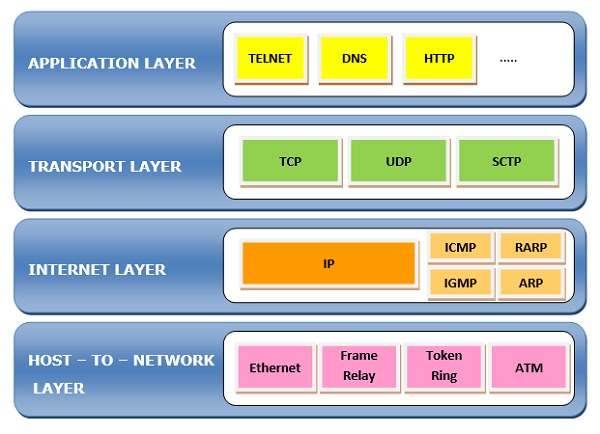
\includegraphics[width=\columnwidth]{tcpip}
\end{figure}
The four layers in the TCP/IP protocol suite are

\begin{enumerate}
  \item \textbf{Host-to-Network Layer}

    It is the lowest layer that is concerned with the physical transmission of
    data. TCP/IP does not specifically define any protocol here but supports
    all the standard protocols.
  \item \textbf{Internet Layer}

    It defines the protocols for logical transmission of data over the network.
    The main protocol in this layer is Internet Protocol (IP) and it is
    supported by the protocols ICMP, IGMP, RARP, and ARP.
  \item \textbf{Transport Layer}
    
    It is responsible for error-free end-to-end delivery of data. The protocols
    defined here are Transmission Control Protocol (TCP) and User Datagram
    Protocol (UDP).
  \item \textbf{Application Layer}
    
    This is the topmost layer and defines the interface of host programs with
    the transport layer services. This layer includes all high-level protocols 
    like Telnet, DNS, HTTP, FTP, SMTP, etc.
\end{enumerate}

\section{Client-server model}
The Client-server model is a distributed application structure that partitions 
task or workload between the providers of a resource or service, called
servers, and service requesters called clients. In the client-server
architecture, when the client computer sends a request for data to the server
through the internet, the server accepts the requested process and deliver the 
data packets requested back to the client. Clients do not share any of their
resources. Examples of Client-Server Model are Email, World Wide Web, etc.
\subsection{Working}

\begin{figure}[h]
  \centering
  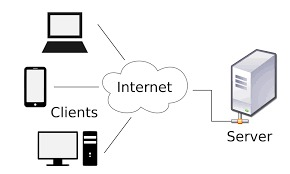
\includegraphics[width=\columnwidth]{cliserv}
\end{figure}

\subsubsection{Client}
When we talk the word Client, it mean to talk of a person or an organization
using a particular service. Similarly in the digital world a Client is a
computer (Host) i.e. capable of receiving information or using a particular
service from the service providers (Servers).
\subsubsection{Servers}
Similarly, when we talk the word Servers, it mean a person or medium that
serves something. Similarly in this digital world a Server is a remote computer
which provides information (data) or access to particular services.

So, its basically the Client requesting something and the Server serving it as 
long as its present in the database.

\begin{figure}[h]
  \centering
  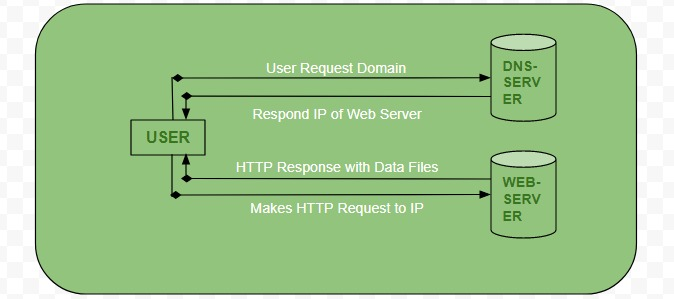
\includegraphics[width=\columnwidth]{serv}
\end{figure}
Advantages of Client-Server model:

\begin{itemize}
  \item Centralized system with all data in a single place.
  \item Cost efficient requires less maintenance cost and Data recovery is
    possible.
  \item The capacity of the Client and Servers can be changed separately.
\end{itemize}

\begin{table}[ht]
  \resizebox{\columnwidth}{!}{
    \begin{tabular}{lp{3.5cm}p{3.5cm}}
      \toprule
      & \textbf{HTTP} & \textbf{HTTPS}\\
      \cmidrule{2-3}
      1 &
        It is hypertext transfer protocol &
        It is hypertext transfer protocol with extra security.\\
      \midrule
      2 &
        It is neither secure or reliable. &
        It is secure and reliable. \\
      \midrule
      3 &
        HTTP URL begins with \texttt{http://} &
        HTTPS URL begins with \texttt{https://} \\
      \midrule
      4 &
        It uses port 80 by default. &
        It uses port 443 by default. \\
      \midrule
      5 &
        It is subjected to man-in-the-middle and evesdropping attacks. &
        It is designed to withstand such attacks and is considered a secure
        option due to this feature. \\
      \bottomrule
    \end{tabular}
  }
  \caption{Difference between HTTP and HTTPS}
\end{table}

\section{Search Engine}
A search engine is a software system designed to carry out web searches. They
search the World Wide Web in a systematic way for particular information
specified in a textual web search query. The search results are generally
presented in a line of results, often referred to as search engine results
pages.

\section{Cookies}
HTTP cookies are small blocks of data created by a web server while a user is
browsing a website and placed on the user's computer or other device by the
user's web browser. Cookies are placed on the device used to access a website,
and more than one cookie may be placed on a user's device during a session.

\section{Webserver}
A web server is computer software and underlying hardware that accepts requests
via HTTP or its secure variant HTTPS. A user agent, commonly a web browser or
web crawler, initiates communication by making a request for a web page or
other resource using HTTP, and the server responds with the content of that
resource or an error message.

\begin{table}[ht]
  \resizebox{\columnwidth}{!}{
    \begin{tabular}{lp{3.5cm}p{3.5cm}}
      \toprule
      & \textbf{Internet} & \textbf{Intranet} \\
      \cmidrule{2-3}
      1 &
        The Internet is a wide network or computers. &
        The Intranet is just a limited network or computers as compared to
        Internet. \\
      \midrule
      2 &
        Internet contains a large number of intranet. &
        Intranet can be accessed from the internet with specific instructions.
        \\
      \midrule
      3 &
        Number of internet users are very high. &
        Number of users is limited. \\
      \midrule
      4 &
        Internet contains various source of information. &
        Intranet only contains group-specific information. \\
      \midrule
      5 &
        Anyone can access the internet. &
        Accessible only by the organization employees or admin who have login 
        details \\
      \midrule
      6 &
        It is not as safe as compared to intranet &
        It is a safe and secure network. \\
      \midrule
      7 &
        It is public by nature. &
        It is private by nature. \\
      \bottomrule
    \end{tabular}
  }
  \caption{Difference between Internet and Intranet}
\end{table}

\newpage
\begin{tcolorbox}
  \part{Unit2}
\end{tcolorbox}
\section{XML DTD (\emph{Document Type Definition})}
A document type definition is a set of markup declarations that define a
document type for an SGML-family markup language. A DTD defines the valid
building blocks of an XML document. It defines the document structure with a
list of validated elements and attributes.

\section{What is markup language?}
Markup language refers to a text-encoding system consisting of a set of
symbols inserted in a text document to control its structure, formatting, or
the relationship between its parts. Markup is often used to control the
display of the document or to enrich its content to facilitating automated
processing.

\section{What is HTML? Features of HTML.}
The HyperText Markup Language or HTML is the standard markup language for
documents designed to be displayed in a web browser. It can be assisted by
technologies such as Cascading Style Sheets (CSS) and scripting languages such
as JavaScript. HTML describes the structure of a webpage. HTML consist of a
series


\section{WML}
Wireless Markup Language, based on XML, is a now-obsolete markup language
intended for devices that implement the Wireless Application Protocol
specification, such as mobile phones. It provides navigational support, data
input, hyperlinks, text and image presentation, and forms, much like HTML.

\newpage
\begin{tcolorbox}
  \part{Unit 3}
\end{tcolorbox}

\section{What is JS variable? How JS variable are declared?}
JS variables are containers for string data values. JS variables can be
declared with the help of `\verb+var+' keyword.
\vskip10pt \noindent\emph{Example}
\begin{verbatim}
var x = 5;
var y = 6;
var z = x+y;
\end{verbatim}

\section{JavaScript Constant}
Constants are immutable variables whose value cannot be changed. Once we have
created a constant, its value cannot be changed.

\begin{verbatim}
var x;
let x; // x is a variable
x = 10; // Integer constant
x = 10.25; // float constant
x = "Ram"; // String constant
x = "R"; // Character constant
x = TRUE; // Boolean constant
\end{verbatim}

\section{What is scripting language? What are the different types of scripting
languages?}
A scripting language is a programming language for a special run-time
environment that automates the execution of tasks; the tasks can alternative
be executed one-by-one by a human operator.

Scripting languages are:
\begin{itemize}
  \item Interpreted rather than compiled.
  \item Used for short scripts over full computer programs.
\end{itemize}
JS, Python, Ruby are all examples of scripting languages.

\begin{table}[ht]
  \resizebox{\columnwidth}{!}{
    \begin{tabular}{lp{3.5cm}p{3.5cm}}
      \toprule
      & \textbf{Client-side scripting} & \textbf{Client-side scripting} \\
      \cmidrule{2-3}
      1 &
        Used when the users browser already has the code. &
        Used to create dynamic pages. \\
      \midrule
      2 &
        The web browser executes the client-side scripting. &
        The web server executes the server-side scripting. \\
      \midrule
      3 &
        Cannot be used to connect to the databases. &
        Used to connect to the databases that reside on the web server. \\
      \midrule
      4 &
        Response from a client-side script is faster as compared to a
        server-side script. &
        Response from a server-side script is slower as compared to a
        client-side script. \\
      \midrule
      5 &
        Can’t access the file system that resides at the web server. &
        Can access the file system residing at the web server. \\
      \midrule
      6 &
        Example of client-side-script are: VB Script, WML Script, Python,
        Action Script, etc. &
        Example of server-side-script are: ASP, JSP, ASP.net, nodejs, PHP,
        SSJS, etc. \\
      \bottomrule
    \end{tabular}
  }
  \caption{Difference between client-side and server-side scripting}
\end{table}

\section{JavaScript Events}
JavaScript events are "things" that happen to HTML elements. When JS is used in HTML
pages, JS can "react" on these events.

\subsection{HTML Events}
An HTML event can be something the browser does, or something a user does.

Here are some examples of HTML events:
\begin{itemize}
  \item An HTML web page has finished loading.
  \item An HTML input field was changed.
  \item An HTML button was clicked.
\end{itemize}
Often, when events happen, you may want to do something. JavaScript lets you
execute code when events are detected. HTML allows event handler attributes,
with JavaScript code, to be added to HTML elements.

\vskip10pt
\noindent With single quotes:
\begin{verbatim}
<element event=`some JavaScript'>
\end{verbatim}
With double quotes:
\begin{verbatim}
<element event="some JavaScript">
\end{verbatim}
In the following example, an onclick attribute (with code), is added to a
\verb+<button>+ element:
\begin{small}
  \begin{verbatim}
<button onclick="document.getElementById('
  demo').innerHTML = Date()">The time is?
</button>
  \end{verbatim}
\end{small}

\subsubsection{Common HTML events}
Refer to \textbf{Table \ref{tab:html-elements}} for the entire list of HTML
elements
\begin{table}
  \resizebox{\columnwidth}{!}{
    \begin{tabular}{lp{4cm}}
      \toprule
      \textbf{Event} & \textbf{Description} \\
      \midrule
      \texttt{onchange} &
        An HTML element has been changed \\
      \midrule
      \texttt{onclick} &
        The user clicks an HTML element \\
      \midrule
      \texttt{onmouseover} &
        The user moves the mouse over an HTML element \\
      \midrule
      \texttt{onmouseout} &
        The user moves the mouse away from an HTML element \\
      \midrule
      \texttt{onkeydown} &
        The user pushes a keyboard key \\
      \midrule
      \texttt{onload} &
        The browser has finished loading the page \\
      \bottomrule
    \end{tabular}
  }
  \caption{Common HTML events}
  \label{tab:html-elements}
\end{table}


\section{Function}
A function is a set of statements that take inputs, do some specific
computation, and produce output. The idea is to put some commonly or
repeatedly done tasks together and make a function so that instead of writing 
the same code again and again for different inputs, we can call that function.

\subsection{Implementation of function in Javascript}
\begin{small}
\begin{verbatim}
function functionName(Param1, Param2, ...)
{
    // Function body
}
\end{verbatim}
\end{small}

\section{Mutable and immutable in Javascript}
A mutable value is one that can be changed without creating an entirely new
value. In JavaScript, objects and arrays are mutable by default, but primitive
values are not -- once a primitive value is created, it cannot be changed,
although the variable that holds it may be reassigned.



\pagebreak
\onecolumn
\section{Write a JavaScript program to find the number is prime or not.}
\section{Write a JavaScript program to find the average of three number (or
average of n number).}
\end{document}
